%!TeX root = Chapter_Method2
\documentclass[../../CompleteThesis2/Complete_2ndDraft]{subfiles}
\graphicspath{{../../Figures/}}
\begin{document}

\section[$\sigma$ Estimation Method][$\sigma$ Estimation Method]{$\sigma$ Estimation Method}
\label{Sec:Method_SigmaMethod}
Usually, when back-diffusing a depth series, some amplitude is regained on the signal, and some peaks and troughs, that might have been washed out from the diffusion might emerge when restoring the signal. These two properties thus makes it possible to connect the diffusion length to the years counted in that section (i.e. the number of peaks and troughs). Due to the knowledge of time passed from the Laki to the Tambora event, the data, along with the restoration techniques, permits a further investigation of the diffusion length in the given section. Thus, when back-diffusing, instead of just using the diffusion length estimate from the spectra, it is possible to examine which diffusion length that results in the correct number of years counted in that section. This property is what will be utilized in the following section, which focuses on finding the optimal diffusion length of a given section.

The general idea of the method is to back diffuse a depth series defined on an interval where the time span (i.e. the number of peaks and troughs expected in that section) is known. The focus is then to find the diffusion length estimate which generates the right number of peaks and troughs in the back diffused depth series. If more than one diffusion length meet these constraints, the largest diffusion length to still fulfill the constraints is sought after. 

The algorithm consists of two modules, where one module describes the numerical back diffusion, given and inputted depth series, core specification and specific $\sigma_0$ estimate (which is either manually inputted or estimated from the spectral analysis). The flowchart describing the processes carried out in this module can be seen in Figure \ref{Fig:FlowchartBackDiffusion}. Many of the sections in this module are only necessary in the initialization of the algorithm as these parts do not change if the inputted diffusion length estimate is changed. In Figure \ref{Fig:FlowchartBackDiffusion} anything carried out above the \textit{Frequency Filters} block to the left is only computed once, and the same with anything to the right of it, except the $\sigma_0$ estimate. The density and diffusion profile calculations, the spectral analysis and the Wiener filter construction is inherent to the depth series alone, and these analyses are carried out as previously described in this thesis.

The second module is responsible for the optimization. This module examines the parameter space containing the diffusion length estimates, and utilizes a direct search method to find the optimal diffusion length estimate.

\begin{figure}
	\begin{tikzpicture}[node distance=1.5cm, auto]
		\node(start) [startstop] {START};
		%----------------------------------------------------%
		\node(in1) [io, left of=start, xshift=-2.5cm] {Depth series};
		\node(empty1) [below of=in1, yshift=0.12cm] {};
		\node(empty2) [below of=in1, xshift=-0.15cm] {};
		%		\node(in1pro1) [process, below of=in1, yshift=-0.5cm] {Spline interpolation};
		\node(in1pro2) [process, below of=in1, yshift=-2cm] {Spectral analysis};
		\node(decSpec1) [decision, below of=in1pro2, scale = 0.8, align=center] {DCT ?\\(Interpolation)};
		\node(decSpec2) [decision, left of=decSpec1, scale=0.8, xshift = -1.2cm, align=center] {FFT ?\\(Interpolation)};
		\node(decSpec3) [decision, right of=decSpec1, scale=0.8, xshift = 0.8cm] {NDCT ?};
		
		\node(in1pro3) [process, below of=decSpec1] {Wiener filter};
		
		\draw[arrow] (in1) -- (start);
		\draw[-] (start) |- (empty2);
		\draw[arrow] (empty1) -- (in1pro2);
		%		\draw[arrow] (in1pro1) -- (in1pro2);
		\draw[arrow] (in1pro2) -- (decSpec1);
		\draw[arrow] (in1pro2) -- (decSpec2);
		\draw[arrow] (in1pro2) -- (decSpec3);
		\draw[arrow] (decSpec1) -- (in1pro3);
		\draw[arrow] (decSpec2) -- (in1pro3);
		\draw[arrow] (decSpec3) -- (in1pro3);
		%	\draw[arrow] (in1pro3) -- (in1pro4);
		
		%----------------------------------------------------%
		
		\node(in2) [io, right of=start, xshift=2.5cm] {Core specs};
		\node(in2pro1) [process, below of=in2, yshift=-0.5cm] {Density profile};
		\node(in2pro2) [process, below of=in2pro1] {Diffusion profile};
		\node(in2pro3) [process, below of=in2pro2] {$\sigma_0$\textbf{ estimate}};
		\node(decSigma1) [decision, below of=in2pro3, scale = 0.8] {$\sigma_0 = \sigma_{\text{const}}$?};
		\node(decSigma2) [decision, right of=decSigma1, scale = 0.8, xshift=0.8cm] {$\sigma_0 = \sigma(z)$?};
		\node(decSigma3) [decision, left of=decSigma1, scale = 0.8, xshift=-0.8cm] {$\sigma_0 = \sigma_{\text{input}}$?};
		
		
		\draw[arrow] (in2) -- (start);
		\draw[arrow] (start) |- (in2pro1);
		\draw[arrow] (in2pro1) -- (in2pro2);
		\draw[arrow] (in2pro2) -- (in2pro3);
		\draw[arrow] (in2pro3) -- (decSigma1);
		\draw[arrow] (in2pro3) -- (decSigma2);
		\draw[arrow] (in2pro3) -- (decSigma3);
		
		%----------------------------------------------------%
		\node(pro0) [process, below of=start, yshift=-6.5cm] {Frequency Filters};
		\node(pro1) [process, below of=pro0,align=center] {\textbf{Deconvolution}\\(Uniform resampling)};
		\node(stop) [startstop, below of=pro1] {\textbf{STOP}};
		\node(out1) [io, right of=stop, align=center, xshift=2.2cm, text width=2.5cm] {\footnotesize{Back diffused depth series}};
		\node(out2) [io, below of=out1, align=center] {\footnotesize{$\sigma_{\text{out}}$}};
		\draw[arrow] (in1pro3) |- (pro0);
		\draw[arrow] (decSigma1) |- (pro0);
		\draw[arrow] (decSigma2) |- (pro0);
		\draw[arrow] (decSigma3) |- (pro0);
		\draw[arrow] (pro0) -- (pro1);
		\draw[arrow] (pro1) -- (stop);
		\draw[arrow] (stop) -- (out1);
		\draw[arrow] (stop) |- (out2);
		
		%		\draw[arrow] (in2pro3) -| (pro0);
		
	\end{tikzpicture}
	\caption[Flowchart of initialization method.]{\small Flowchart of initialization method for back diffusion of a depth series given a diffusion length estimate.}
	\label{Fig:FlowchartBackDiffusion}
\end{figure}


\subsection[Corrections on $\sigma$][Corrections on $\sigma$]{Corrections on the Computed $\sigma$ estimate}
\label{Subsec:Method_SigmaMethod_SigmaCorrections}
As mentioned in Section \ref{Subsec:Ice_DiffusionAndDensification_Diffusion_TemperatureRecon}, the estimated diffusion length needs to be corrected for a number of different influences: the sampling diffusion, the ice diffusion at a given depth and the thinning function at a given drill site.

This section will describe how each of these influences have been taken care of in the work.

\subsubsection{Ice Diffusion, $\sigma_{\text{ice}}$}
\label{Subsubsec:Method_SigmaMethod_SigmaCorrections_IceDiffusion}

\subsubsection{Sampling Diffusion, $\sigma_{\text{dis}}$}
\label{Subsubsec:Method_SigmaMethod_SigmaCorrections_SamplingDiffusion}

\subsubsection{Thinning Function $S(z)$}
\label{Subsubsec:Method_SigmaMethod_SigmaCorrections_ThinningFct}



\subsection[Constraints][Constraints]{Constraints}
\label{Subsec:Method_SigmaMethod_Constraints}
This section will contain a walk through of the general differences between constrained and non-constrained optimization of the diffusion length. In Figure \ref{fig:SiteB_ConstVNoConst} an example of the results of the optimization with and without constraints can be seen.
\begin{figure}[h]
	\centering
	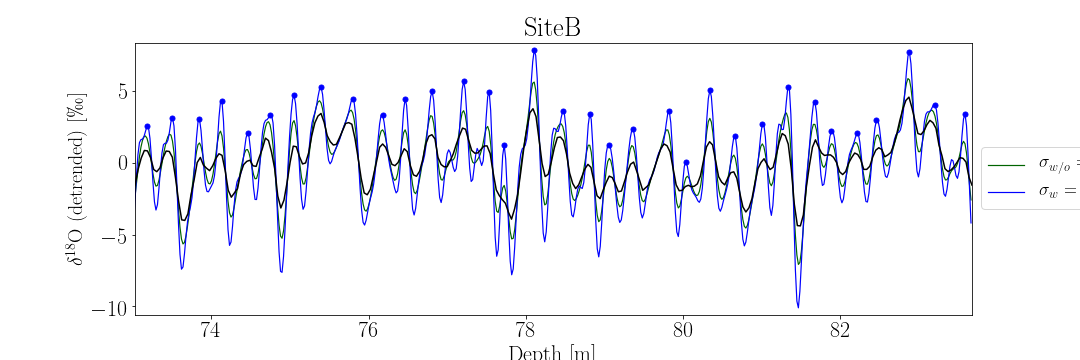
\includegraphics[width=0.95\textwidth]{SiteB_ConstVNoConst.png}
	\caption[Site B Constrained vs. Unconstrained]{\small Example of how the imposed constraints effect the final diffusion length estimate for the Laki to Tamborad depth section of the core drilled at Site B. The black line shows the data, the green the back diffused data using a method with less constraints, and the blue shows the back diffused data when using the imposed constraint. The blue dots represents the peaks counted in the constrained method.}
	\label{fig:SiteB_ConstVNoConst}
\end{figure}


%\subsection[$1^{\text{st}}\sigma$ Estimate][$1^{\text{st}}\sigma$ Estimate]{$1^{\text{st}}$ Diffusion Length Estimate}
%\label{Subsec:Method_SigmaMethod_1stEstimate}

%\subsection[Optimal $\sigma$ Estimate][Optimal $\sigma$ Estimate]{Optimal Diffusion Length Estimate}
%\label{Subsec:Method_SigmaMethod_OptEstimate} 


\section[Testing and Stability][Testing and Stability]{Method Testing and Stability}
\label{Sec:Method_TestStab}

Throughout this section a number of different tests of the algorithm will be presented. The tests are performed to examine the stability of the method, the accuracy of the Laki and Tambora positions and how the choice of parameters(interpolation, spectral transform type, ALT estimation, peak prominence and peak distance) changes the resulting diffusion length estimate. 

\subsection[Constraints or No Constraints]{No constraints versus constraints}
\label{Subsec:Method_TestStab_ConstNoConst}


\subsection[ALT Estimation]{Annual Layer Thickness Estimations}
\label{Subsec:Method_TestStab_ALTest}

\begin{figure}[h]
	\centering
	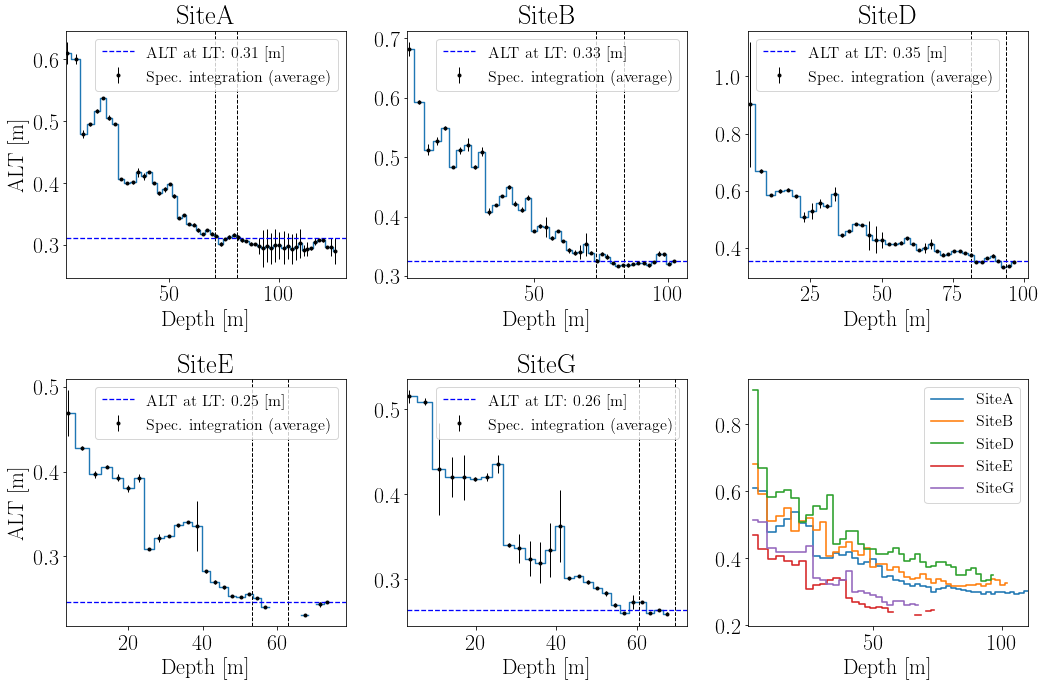
\includegraphics[width=0.95\textwidth]{AllCores_ALTs.png}
	\caption[$\lambda$ for Full Cores]{\small Annual layer thickness estimates, $\lambda$, calculated through spectral integration of 5 m sections of the entire core lengths. The average is based on using both FFT, DCT and NDCT spectral estimations. Blank spaces, akin to the sections below 60 m depth at Site E shows problematic areas, where the spectral estimation have had trouble with determining $\lambda$. The black vertical lines show the depth sections between Laki and Tambora events.}
	\label{fig:AllCores_ALTs}
\end{figure}


\subsubsection[Change in $l_{sec}$]{Change in section length}
\label{Subsubsec:Method_TestStab_ALTest_ChangeLsec}

\begin{figure}[h]
	\centering
	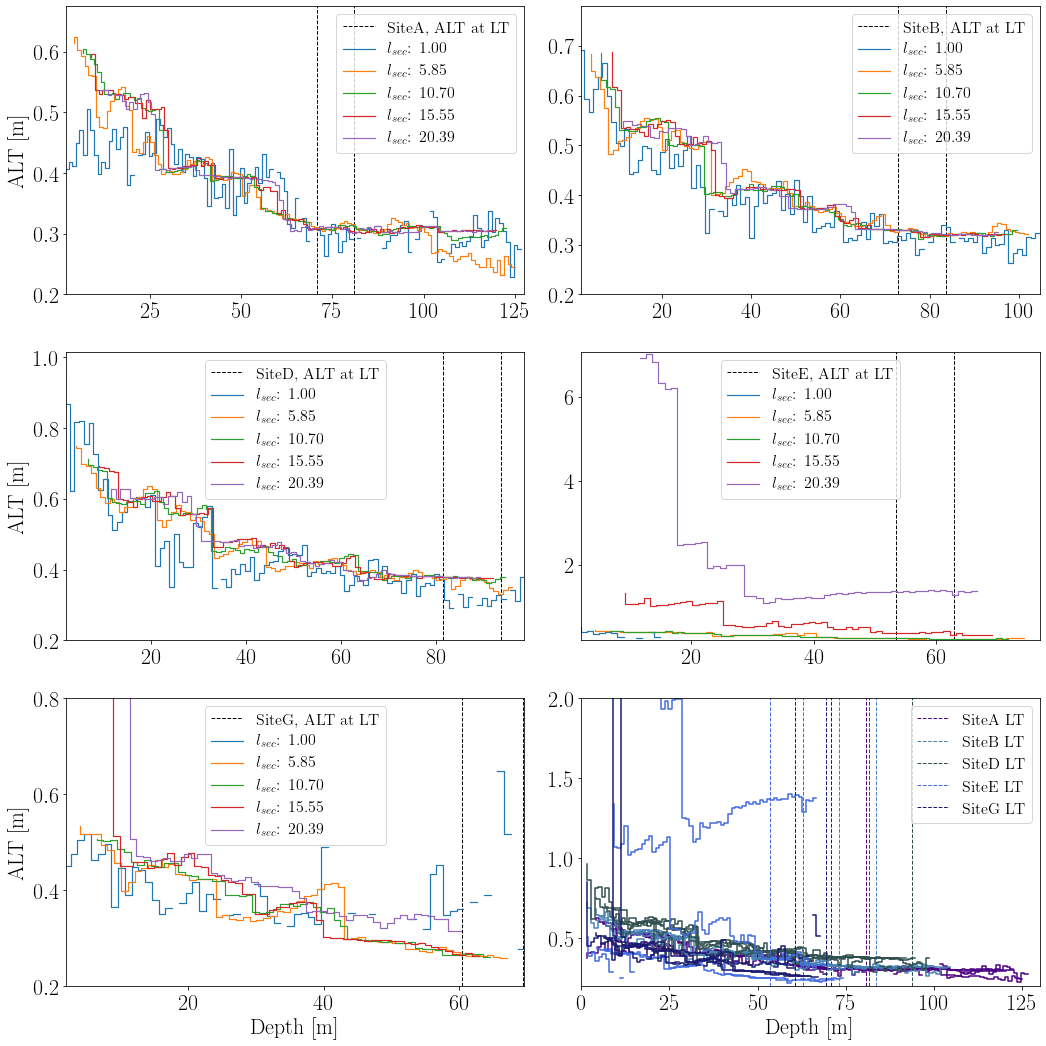
\includegraphics[width=0.95\textwidth]{AllCores_ALT_at_DiffLsecs.png}
	\caption[$\lambda$ Depth Profiles, Different $l_{\text{sec}}$]{\small Examples of the $\lambda$ depth profile given different section lengths. All profiles are computed with a shift of 1 m.}
	\label{fig:AllCores_ALT_at_DiffLsecs}
\end{figure}

\begin{figure}[h]
	\centering
	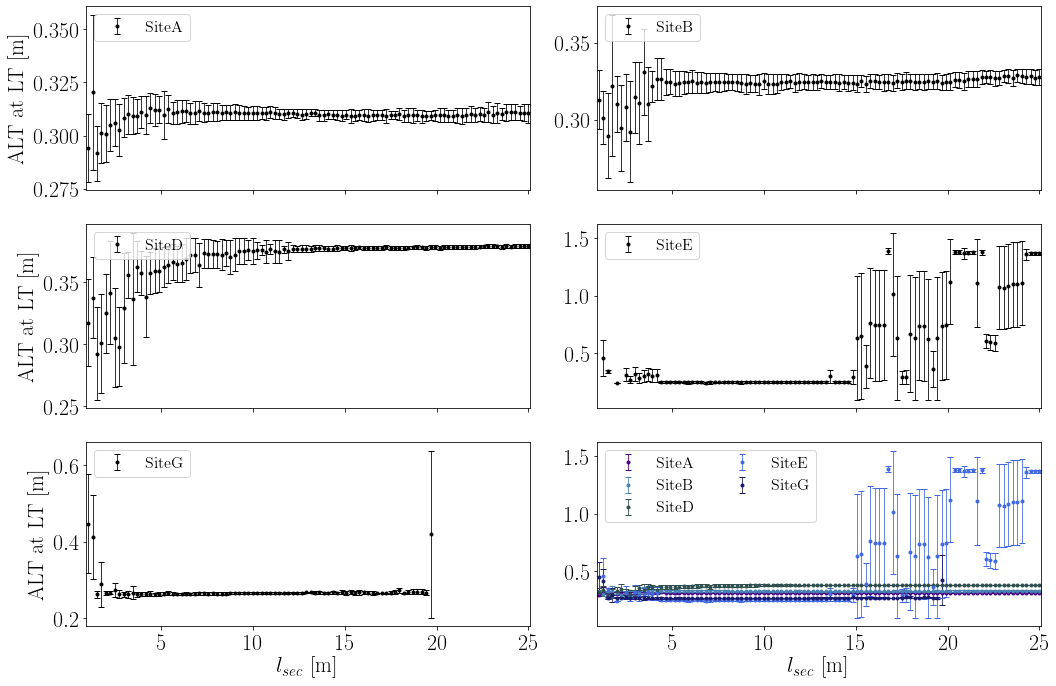
\includegraphics[width=0.95\textwidth]{AllCores_ALTatLT_vs_lSec.png}
	\caption[$\lambda_{\text{LT}}$ vs. Section Length]{\small The annual layer thickness estimates in the section between Laki and Tambora as computed with different section lengths, $l_{\text{sec}}$, used in the spectral analysis. The section is shifted 1 m and then computed again. The $\lambda_{\text{LT}}$ is then calculated as a mean of th $\lambda$ estimates falling into the Laki to Tambora depth section.}
	\label{fig:AllCores_ALTatLT_vs_lSec}
\end{figure}




\subsubsection[Change in $l_{shift}$]{Change in shift length}
\label{Subsubsec:Method_TestStab_ALTest_ChangeLshift}

\begin{figure}[h]
	\centering
	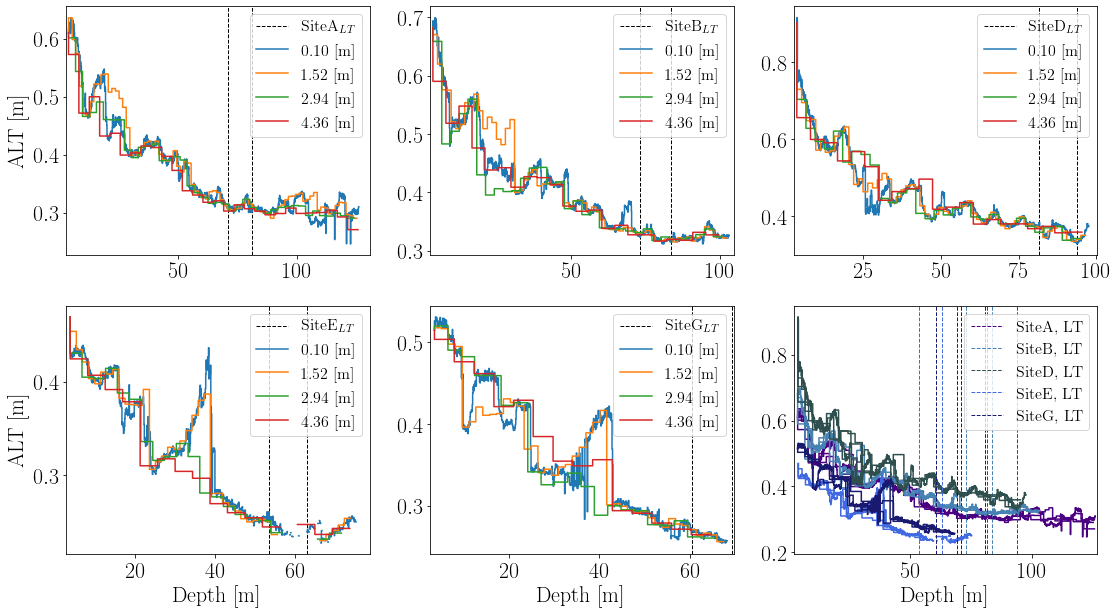
\includegraphics[width=0.95\textwidth]{AllCores_ALT_at_DiffShifts.png}
	\caption[$\lambda$ Depth Profiles, Different $s_{\text{sec}}$]{\small Examples of $\lambda$ depth profiles given different shift lengths. All profiles are computed with a section length for spectral analysis of $l_{\text{sec}}=5$ m.}
	\label{fig:AllCores_ALT_at_DiffShifts}
\end{figure}


\begin{figure}[h]
	\centering
	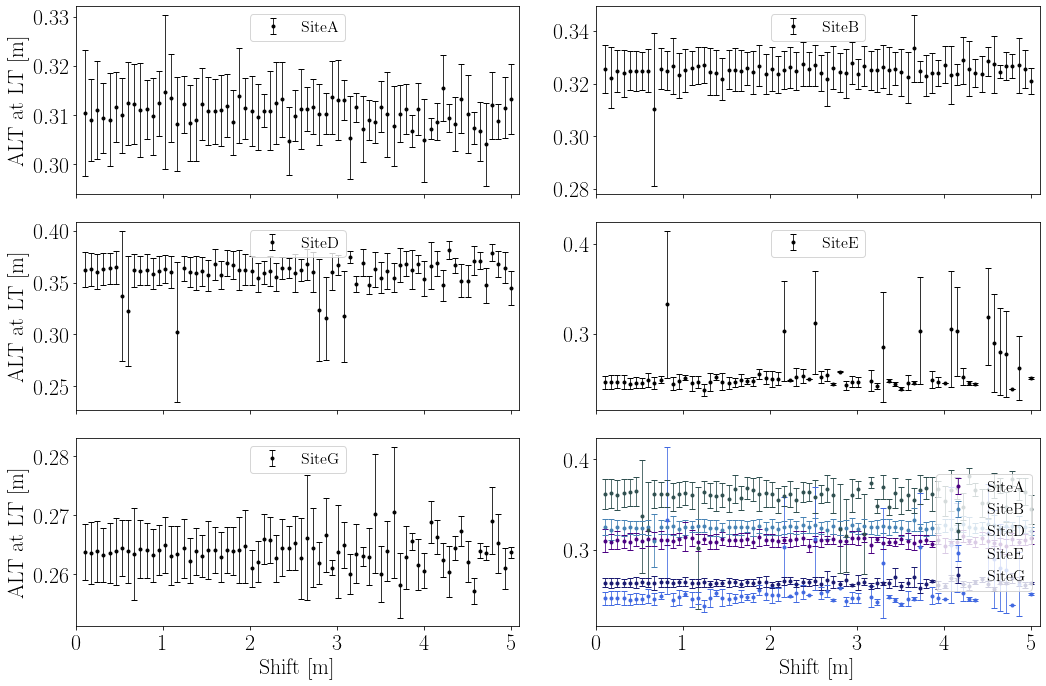
\includegraphics[width=0.95\textwidth]{AllCores_ALTvsShift.png}
	\caption[$\lambda_{\text{LT}}0$ vs. $s_{\text{sec}}$]{\small Annual layer thickness estimate at the depth section between Laki and Tambora, $\lambda_{\text{LT}}$ versus different shifts of the sections used in the spectral analysis.}
	\label{fig:AllCores_ALTvsShift}
\end{figure}



\subsection[Spectral Transforms]{Spectral Transform's Effect on Diffusion Length}
\label{Subsec:Method_TestStab_SpecTrans}

\subsubsection{Visual Inspection}
\label{Subsubsec:Method_TestStab_SpecTrans_VisInspection}

\begin{figure}[h]
	\centering
	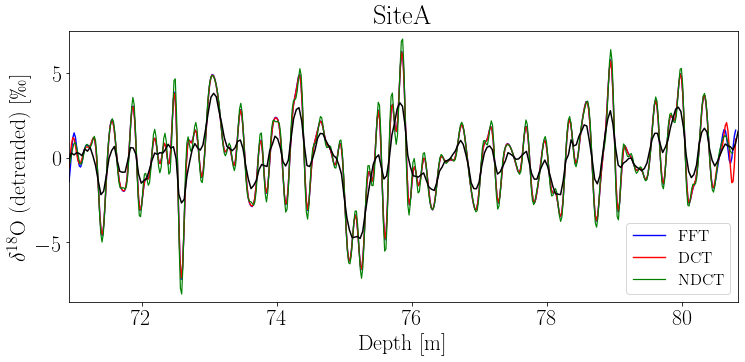
\includegraphics[width=0.8\textwidth]{SiteA_SpecTrans_VisInspection.png}
	\caption[Qualitative Example of Spectral Transform's Effect on $\sigma$]{\small A visual example of the differences in final back diffused data when using different spectral transforms. }
	\label{fig:SiteA_SpecTrans_VisInspection}
\end{figure}


\subsubsection{Speed Examination}
\label{Subsubsec:Method_TestStab_SpecTrans_Speed}

\begin{figure}[h]
	\centering
	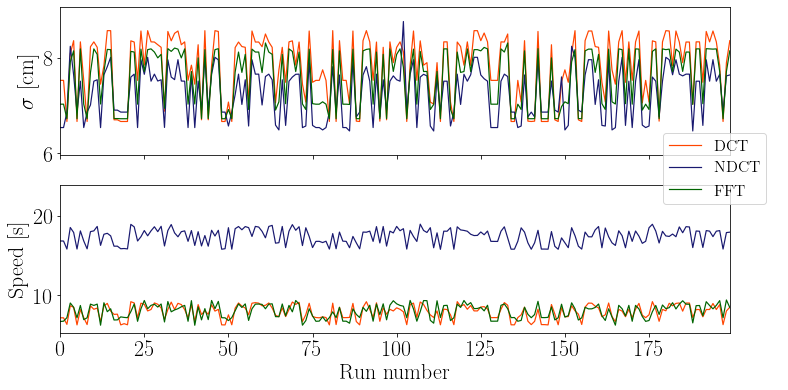
\includegraphics[width=0.95\textwidth]{SiteA_SpecTrans_Speed.png}
	\caption[Speed and $\sigma$ Estimates, Spectral Transforms]{\small Diffusion length estimate along with speed of algorithm given the three different spectral transforms examined in this work. The volcanic event depths have been drawn from a Gaussian distribution with a width corresponding to ~1 month around the estimated mean depth of the event.}
	\label{fig:SiteA_SpecTrans_Speed}
\end{figure}




\subsection[LT locations]{Laki and Tambora as Gaussian Distributions}
\label{Subsec:Method_TestStab_LTlocations}



\subsubsection[Vary L and T]{Varying both Laki and Tambora Position}
\label{Subsubsec:Method_TestStab_LTlocations_LandT}

\begin{figure}[h]
	\centering
	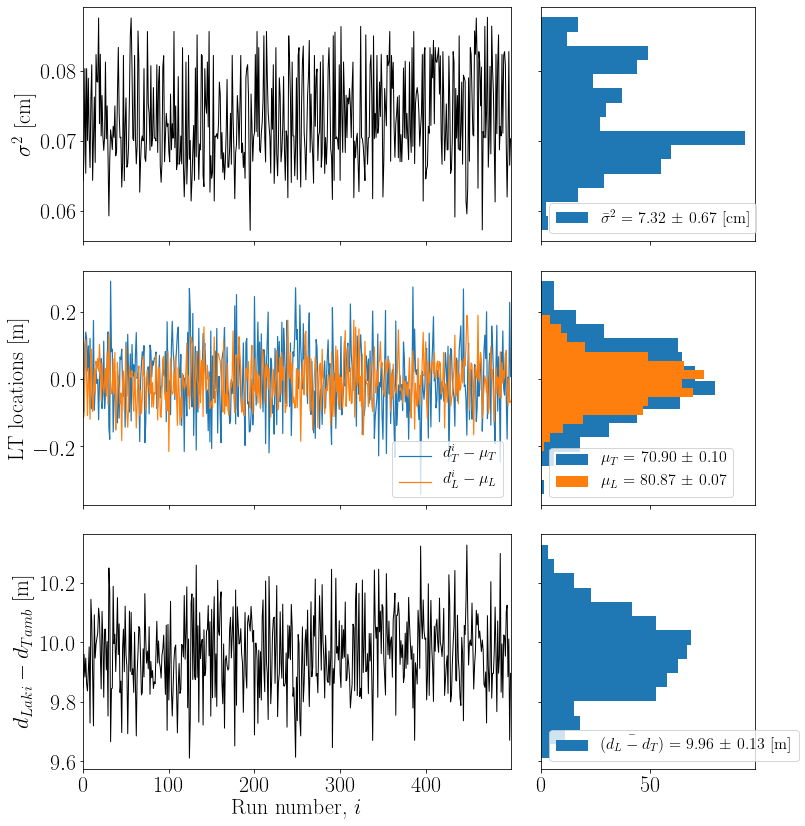
\includegraphics[width=0.95\textwidth]{SiteA_Vary_LandT.png}
	\caption[Diffusion Length Variations, Varying Laki and Tambora]{\small Diffusion length estimates when varying the depth locations of the volcanic events. The locations of both Laki and Tambora events have been drawn from Gaussian distributions as the ones presented in Section \ref{Sec:Data_VolcanicHorizons}.}
	\label{fig:SiteA_Vary_LandT}
\end{figure}



\subsubsection[Vary T]{Varying only Tambora Position}
\label{Subsubsec:Method_TestStab_LTlocations_T}

\begin{figure}[h]
	\centering
	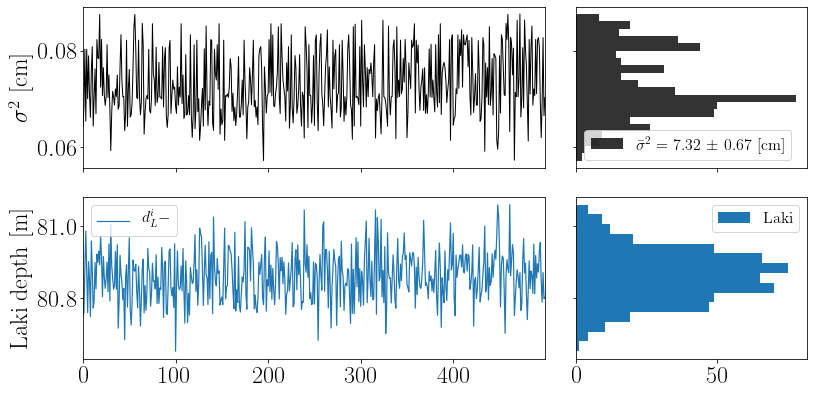
\includegraphics[width=0.95\textwidth]{SiteA_Vary_Lonly.png}
	\caption[Diffusion Length Variations, Varying only Laki]{\small Diffusion length estimates for Site A when varying only the Laki volcanic event. The locations are drawn from Gaussian distributions as the ones presented in Section \ref{Sec:Data_VolcanicHorizons}. The depth section is kept at a constant length, corresponding to the mean distance value, $\bar{d}_{\text{Laki}}-\bar{d}_{\text{Tambora}}$.}
	\label{fig:SiteA_Vary_Tonly}
\end{figure}



\subsubsection[Vary L]{Varying only Laki Position}
\label{Subsubsec:Method_TestStab_LTlocations_L}

\begin{figure}[h]
	\centering
	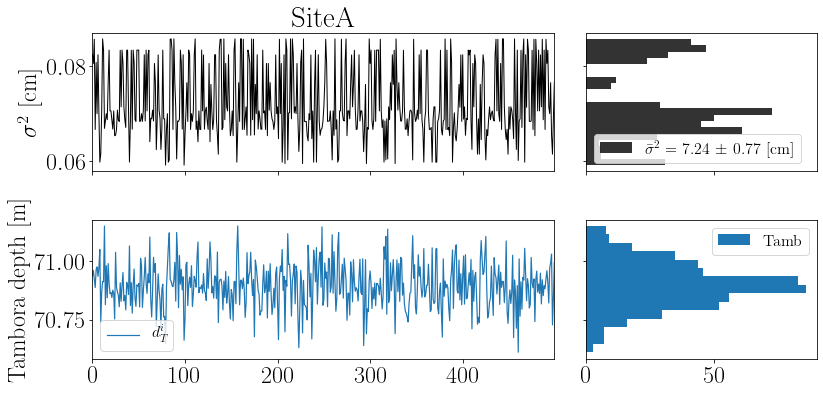
\includegraphics[width=0.95\textwidth]{SiteA_Vary_Tonly.png}
	\caption[Diffusion Length Variations, Varying only Tambora]{\small Diffusion length estimates for Site A when varying only the Tambora volcanic event. The locations are drawn from Gaussian distributions as the ones presented in Section \ref{Sec:Data_VolcanicHorizons}. The depth section is kept at a constant length, corresponding to the mean distance value, $\bar{d}_{\text{Laki}}-\bar{d}_{\text{Tambora}}$.}
	\label{fig:SiteA_Vary_Lonly}
\end{figure}



\subsubsection[2 Month Variability]{Variation Corresponding to 2 Months}
\label{Subsubsec:Method_TestStab_LTlocations_2Month}

\begin{figure}[h]
	\centering
	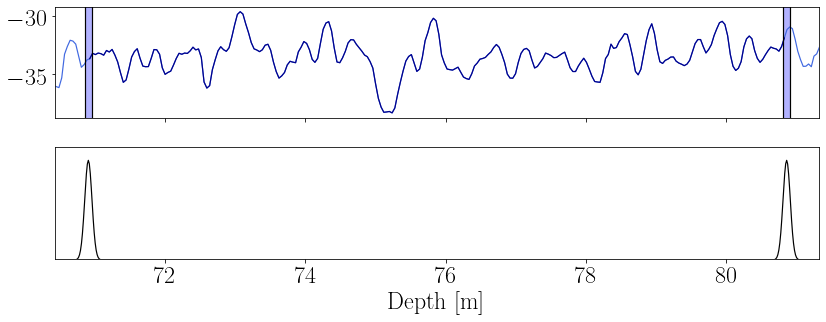
\includegraphics[width=0.95\textwidth]{SiteA_LandT_Gauss_2Mnth.png}
	\caption[Illustration of 2 Month Standard Deviation Variation of Volcanic Events Locations]{\small Illustration of the method implemented to manage the uncertainty of the exact depth location of the volcanic events. The method establishes a Gaussian distribution with a mean of the estimated middle of the volcanic event and a standard deviation of what corresponds to two months.}
	\label{fig:SiteA_LandT_Gauss_2Mnth}
\end{figure}

%\begin{figure}[h]
%	\centering
%	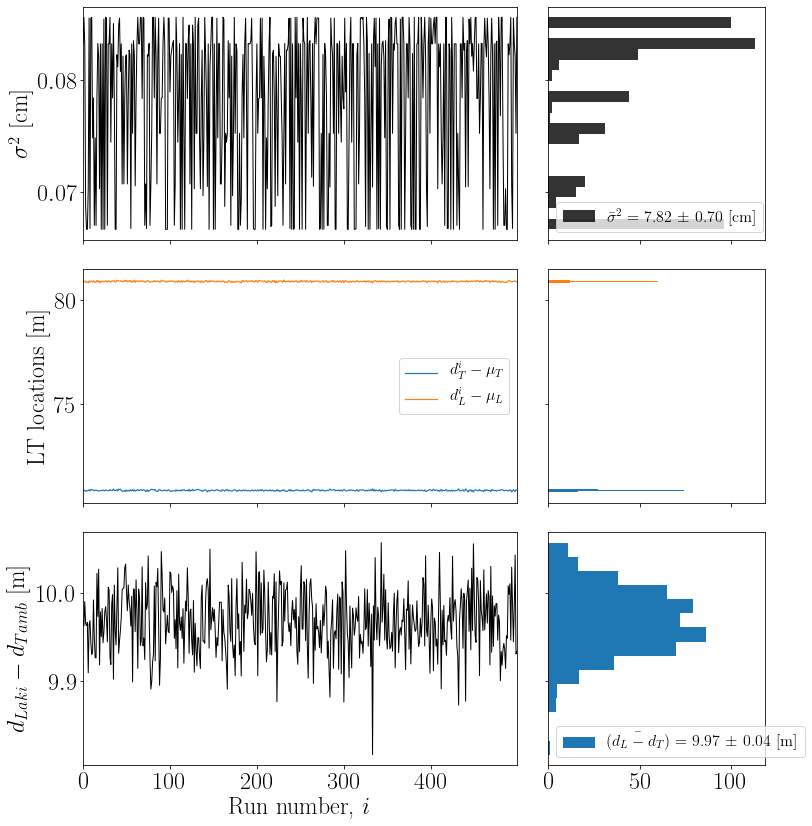
\includegraphics[width=0.95\textwidth]{SiteA_Vary_LandT_2mnth_DCT.png}
%	\caption[2 Month Variation of Event Locations, Site A]{\small 500 runs with locations of Laki and Tambora events drawn from a Gaussian distribution with a standard deviation of two months. Using DCT as spectral transform.}
%	\label{fig:SiteA_LandT_Gauss_2mnth_DCT}
%\end{figure}

\begin{figure}[h]
	\centering
	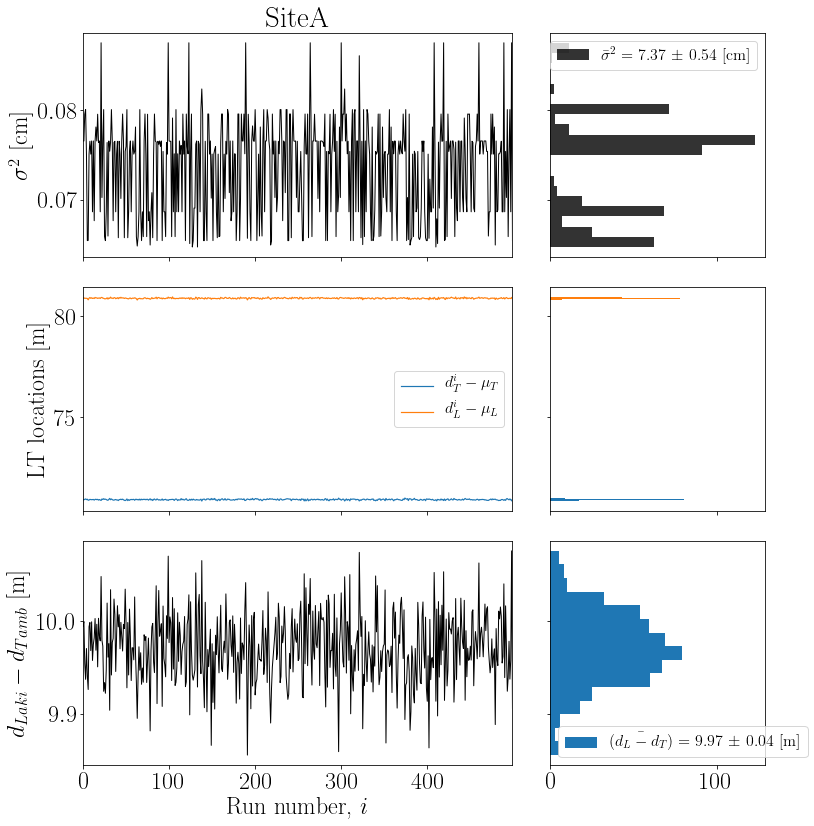
\includegraphics[width=0.95\textwidth]{SiteA_Vary_LandT_2mnth_NDCT.png}
	\caption[2 Month Variation of Event Locations, Site A]{\small 500 runs with locations of Laki and Tambora events drawn from a Gaussian distribution with a standard deviation of two months. Using NDCT as spectral transform.}
	\label{fig:SiteA_LandT_Gauss_2mnth_NDCT}
\end{figure}



\section[Upgrades][Upgrades]{Possible Algorithms Upgrades}
\label{Sec:Method_Upgrades}

This section will discuss ideas on how to improve on both the method and the algorithm

\subsection[Peak Detection]{Peak Detection}
\label{Subsec:Method_Upgrades_PeakDet}

\subsection[Optimization Routine]{Optimization Routine}
\label{Subsec:Method_Upgrades_OptiRout}









\end{document}
